\section{Sample slides}
\subsection{Theory}
\begin{frame}{Some maths}
  Maths fonts can be set in \texttt{beamerthemetudo.sty} or \texttt{beamerthemetudo\_dark.sty}.
  Currently this is set to \enquote{Latin Modern Math}. Look for \texttt{\textbackslash setmathfont\{\}}
  to set a different math font.
  \begin{align*}
    \nabla \cdot \vec{B} &= 0 &
    \nabla \cdot \vec{E} &= \frac{ρ}{ε_0} \\
    \nabla \times \vec{E} &= -\partial_t \vec{B} &
    \nabla \times \vec{B} &= μ_0 \vec{j} + μ_0 ε_0 \partial_t \vec{E} &
  \end{align*}
\end{frame}

\subsection{Results}
\begin{frame}{Plot}
    This theme also comes with a \texttt{darkmode.mplstyle} that allows you to create
    plots fitting the dark or light theme (see \texttt{plots/darkmode.mplstyle}). The style will
    be applied automatically when running \texttt{make <all | light | dark>}.
  \begin{figure}
    \centering
    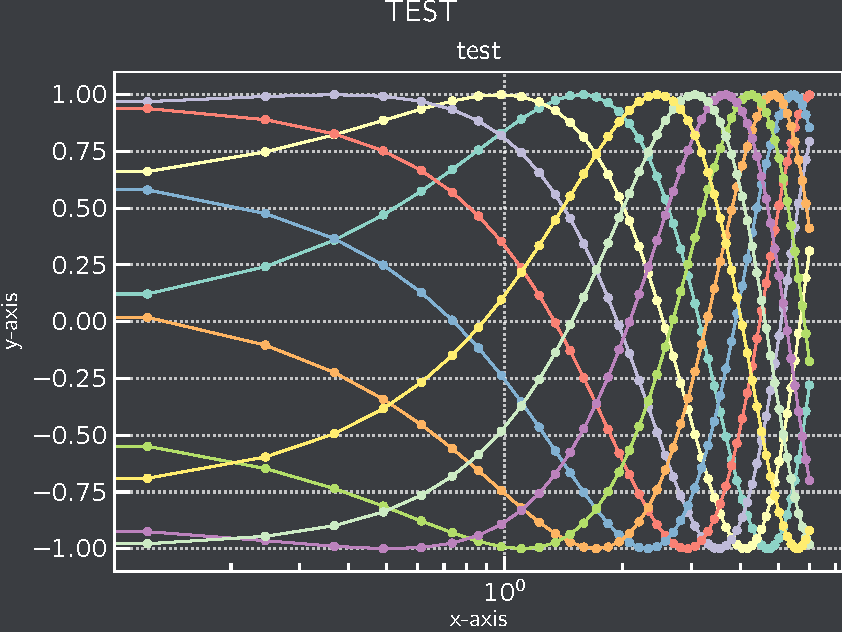
\includegraphics[height=0.75\textheight]{plots/plot.pdf}
  \end{figure}
\end{frame}